\section{Popiště model diskrétního kanálu s poruchami, čím se liší od ideálního kanálu}
\begin{itemize}
    \item Vstup poruch do kanálu způsobí, že při vysílání prvku $x_i$ se může změnit na prvek $y_j$.
    Nese-li prvek $x_i$ informaci I$(x_i)$, pak změni budeme vyjadřovat jako
    $$\mathrm{I}(x_i, y_j) = \mathrm{I}(x_i / y_j$$
    \item Od ideálního kanálu se liší tím, že v ideálním kanále je provozními podmínkami zajištěno, že nemusíme brát v úvahu působení chyb
\end{itemize}

\section{Uveďte AWGN model přenosu spojitým kanálem}
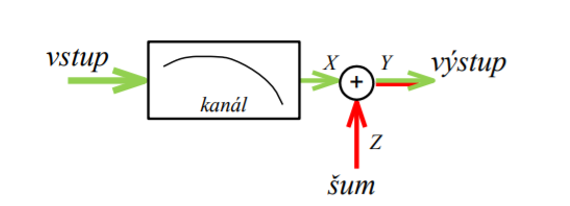
\includegraphics[]{images/AWGN.png}

\section{Uveďte a popište Shannonův vztah pro kapacitu kanálu. Za jakých podmínek byl odvozen: model, charakter signálu a šumu, Co je SNR a jak se většinou udává?}
$$C = B*log_2(1+SNR)$$.
Byl odvozen za podmínek platnosti Nyquistova kritéria.
$$M \leqq 2B$$, které říká, že potřebná šířka pásma je B je minimálně poloviční oproti modulační rychlosti M, anebo opačně maximální modulační rychlost M je rovna dvojnásobku šířky pasma.

\textbf{SNR} znamená tzv. odstup signál šum na straně přijámače, jednotka jsou decibely [dB]

\section{Co je to modulační rychlost? Jakou má jednotku? Jaký je vztah mezi ní a šiřkou pásma}
viz. otázka 8.

Vztah mezi modulační rychlostí a šiřkou pásma
\begin{itemize}
    \item Pro spojitý kanál je popsán nyquistovým kritériem
    \item $M \leqq 2B $, které říká, že potřebná šířka pásma B je minimálně poloviční oproti modulační rychlosti M anebo opačně maximální modulační rychlost M je rovna dvojnásobku šířky pásma.
\end{itemize}

\section{Co popisuje výkonová spektrální hustota, jakou má jednotku, v jakých jednotkách se zpravidla udává. Uveďte vztah pro výkon}
\begin{itemize}
    \item Výkonová spektrální hustota popisuje rozložení výkonu napříč spektrem, Její základndí jednotkou je W/Hz. Většinou se ale uvádí v dBm/hz
\end{itemize}
Vzath pro výkon
$$P = \int_{-\infty}^{\infty} PSD(f)\mathrm{d}f$$

\section{Co je to problém příjemce}
Problém příjemce je zjištění, zda platí rovnost $S=S^*, $ kde S=${s_i}$ ze zdroje dat a $S^*$ je vstupní abeceda dekóderu.¨

\section{Co je to „Kódování zdroje“ a „Kódování kanálu“ }
\begin{itemize}
    \item Kódování zdroje -Představitelem tohoto typu kódování je kódování pro přizpůsobení zdroje na kanál z důvodu vyjádření velkého počtu zpráv určujících zdroj zpráv počtem stavů signálu přenositelného kanálem. Existují ale i jiné druhy kódování zdroje
    \item Kódování kanálu - Je spojeno s vlastnostmi kanálu, který slouží k přenosu zprávy kanálem v podobě signálových prvků. K tomuto druhu kódování patří např. protichybové kódování, linkové kódy, modulace a další.
\end{itemize}

\section{Přehled druhů kódování v systémech pro přenos informace a jejich stručný popis}
\begin{itemize}
    \item  Kódy pr přizpůsobení zdroje na kanál - spojeny s realizací přenosového systému a musí být určeno
\begin{itemize}
    \item Definice vlastního kódu
    \item Definice způsobu přiřazení
\end{itemize}
\item Kódy pro snižování nadbytečnosti - některé kódy vytváří zprávy s vysokou redundancí = snižují přenosový výkon systému pro přenos informace. Řešení spočívá v přechodu na jinou, účinnější, abecedu zdroje.
\item Kódy pro zabezpečeení přenosu proti chybám
\item Kódy pro zrovnoměrnění spektra přenášenohé signálu - Scrambling
\item Kódy pro zabezpečení přenosu informace proti zcizení - šifrování
\end{itemize}